%solver
%+++++++++++++++++++++++++++++++++++++++++++++++++++++++++++++++++++++++++++++
%+++++++++++++++++++++++++++++++++++++++++++++++++++++++++++++++++++++++++++++
\mysection{Notation and System of equations of motion}
\label{sec:notationSystemOfEOM}
%
The general idea of the code is to have objects, which provide equations (ODE2, ODE1, AE).
The solver then assembles these equations and solves the static or dynamic problem.
The system structure and solver follow partially the previous implementation in HOTINT \cite{GerstmayrStangl2004,Gerstmayr2009,GerstmayrEtAl2013}.

\mysubsection{LHS-RHS naming conventions in EXUDYN} \label{eq_equationLHSRHS}

Functions and variables contain the abbreviations LHS ({\it left-hand-side}) and RHS ({\it right-hand-side}), sometimes lower-case, in order
to distinguish if terms are computed at the LHS or RHS.

The objects have the following LHS--RHS conventions:
\bi
		\item the acceleration term, e.g., $m \cdot \ddot q$ is always positive on the LHS
	  \item objects, connectors, etc., use LHS conventions for most terms: mass, stiffness matrix, elastic forces, damping, etc., are computed at LHS of the object equation
		\item object forces are written at the RHS of the object equation
		\item in case of constraint or connector equations, there is no LHS or RHS, as there is no acceleration term. 
		Therefore, the computation function evaluates the term as given in the description of the object, adding it to the LHS.
\ei
Object equations may read, e.g., for one coordinate $q$, mass $m$, damping coefficient $d$, stiffness $k$ and applied force $f$,
\be
  \underbrace{m \cdot \ddot q + d \cdot \dot q + k \cdot q}_{LHS} = \underbrace{f}_{RHS}
\ee 
In this case, the C++ function \texttt{ComputeODE2LHS(const Vector\& ode2Lhs)} will compute the term
$d \cdot \dot q + k \cdot q$ with positive sign. Note that the acceleration term $m \cdot \ddot q$ is computed separately, as it 
is computed from mass matrix and acceleration.

However, system quantities (e.g.\ within the solver) are always written on RHS\footnote{except for the acceleration $\times$ mass matrix and constraint reaction forces, see \eq{eq_system_EOM}}: 
\be 
  \underbrace{M_{sys} \cdot \ddot q_{sys}}_{LHS} = \underbrace{f_{sys}}_{RHS} \,.
\ee
In the case of the object equation
\be
  m \cdot \ddot q + d \cdot \dot q + k \cdot q = f \, ,
\ee 
the RHS term becomes $f_{sys} = -(d \cdot \dot q + k \cdot q) + f $ and it is computed by the C++ function \texttt{ComputeSystemODE2RHS}.
%
This means, that during computation, terms which appear at the LHS of the object are transferred to the RHS of the system equation.
This enables a simpler setup of equations for the solver.

\mysubsection{System assembly}
Assembling equations of motion is done within the C++ class \texttt{CSystem}, see the file \texttt{CSystem.cpp}.
The general idea is to assemble, i.e.\ to sum up, (parts of) residuals attributed by different objects. The summation process is based on coordinate indices to which the single equations belong to.
Let's assume that we have two simple \texttt{ObjectMass1D} objects, with object indices $o0$ and $o1$ and having mass $m_0$ and $m_1$. They are connected to nodes of type \texttt{Node1D} $n0$ and $n1$, with global coordinate indices $c0$ and $c1$.
The partial object residuals, which are fully independent equations, read
\bea
  m_0 \cdot \ddot q_{c0} &=& RHS_{c0} \eqComma \\
  m_1 \cdot \ddot q_{c1} &=& RHS_{c1} \eqComma
\eea
where $RHS_{c0}$ and $RHS_{c1}$ the right-hand-side of the respective equations/coordinates. They represent forces, e.g., from \texttt{LoadCoordinate} items (which directly are applied to coordinates of nodes), say $f_{c0}$ and $f_{c1}$, that are in case also summed up on the right hand side.
Let us for now assume that 
\be
  RHS_{c0} = f_{c0} \quad \mathrm{and} \quad RHS_{c1} = f_{c1} \eqDot
\ee

Now we add another \texttt{ObjectMass1D} object with object index $o2$, having mass $m_2$, but letting the object {\it again} use node $n0$ with coordinate $c0$.
In this case, the total object residuals read
\bea
  (m_0+m_2) \cdot \ddot q_{c0} &=& RHS_{c0} \eqComma \\
  m_1 \cdot \ddot q_{c1} &=& RHS_{c1} \eqDot
\eea 
It is clear, that now the mass in the first equation is increased due to the fact that two objects contribute to the same coordinate. The same would happen, if several loads are applied to the same coordinate.

Finally, if we add a \texttt{CoordinateSpringDamper}, assuming a spring $k$ between coordinates $c0$ and $c1$, the RHS of equations related to $c0$ and $c1$ is now augmented to
\bea
  RHS_{c0} &=& f_{c0} + k \cdot (q_{c1} - q_{c0}) \eqComma \\
  RHS_{c1} &=& f_{c1} + k \cdot (q_{c0} - q_{c1}) \eqDot
\eea
The system of equation would therefore read
\bea
  (m_0+m_2) \cdot \ddot q_{c0} &=& f_{c0} + k \cdot (q_{c1} - q_{c0}) \eqComma \\
  m_1 \cdot \ddot q_{c1}  &=& f_{c1} + k \cdot (q_{c0} - q_{c1}) \eqDot
\eea
It should be noted, that all (components of) residuals ('equations') are summed up for the according coordinates, and also all contributions to the mass matrix. 
Only constraint equations, which are related to Lagrange parameters always get their 'own' Lagrange multipliers, which are automatically assigned by the system and therefore independent for every constraint.
Therefore, it is not possible right now to attach two \texttt{ObjectRigidBody}  to the same node, as it would create two constraint equations. This will be resolved within issue \#0564.

\mysubsection{Nomenclature for system equations of motion and solvers}
\label{sec:nomenclatureEOM}
%Nomenclature:
%\bi
	%\item '\SO' $\ldots$ second order equations (usually of a mechanical system)
	%\item '\FO' $\ldots$ first order equations (e.g.\ of a controller, fluid, etc.)
	%\item '$\AE$' $\ldots$ algebraic equations (usually of joints)
	%%
%\ei
%\newcommand{\acc}{\av} %avoid due to possible mix up with algorithmic acceleration
\newcommand{\aalg}{\av} 
\newcommand{\vel}{\vv} %use this for transformation of ODE2 into first order equations
Using the basic notation for coordinates in \refSection{sec:itemnotation}, we use the following quantities and symbols for equations of motion and solvers:
\begin{center}
  \footnotesize
  \begin{longtable}{| p{5cm} | p{5cm} | p{6cm} |}
    \hline
    \bf quantity & \bf symbol & \bf description \\ \hline
%
    number of ODE2 coordinates & $n$ & ODE2 = \SON \\ \hline
    number of ODE1 coordinates & $n_\FO$ & ODE1 = \FON \\ \hline
    number of AE coordinates & $m$ & AE = \AEN \\ \hline
    number of system coordinates & $n_{\SYS}$ & \SYSN \\ \hline
%
    ODE2 coordinates & $\qv = [q_0,\, \ldots,\, q_{n_q}]\tp$ & ODE2, displacement-based coordinates (could also be rotation or deformation coordinates)\\ \hline
		%\vel needed for transformation to first order equations
    ODE2 velocities & $\vel = \dot \qv = [\dot q_0,\, \ldots,\, \dot q_{n_q}]\tp$ & ODE2 velocity coordinates\\ \hline
    ODE2 accelerations & $\ddot \qv = [\ddot q_0,\, \ldots,\, \ddot q_{n_q}]\tp$ & ODE2 acceleration coordinates\\ \hline
    ODE1 coordinates & $\yv = [y_0,\, \ldots,\, y_{n_y}]\tp$ & vector of $n_y$ coordinates for first order ordinary differential equations (ODE1)\\ \hline
    ODE1 velocities & $\dot \yv = [\dot y_0,\, \ldots,\, \dot y_{n_y}]\tp$ & vector of $n$ velocities for first order ordinary differential equations (ODE1)\\ \hline
%currently not used/needed:    algebraic coordinates & $\zv = [z_0,\, \ldots,\, z_m]\tp$ & vector of $m$ algebraic coordinates if not Lagrange multipliers in any configuration\\ \hline
    ODE2 Lagrange multipliers & $\tlambda = [\lambda_0,\, \ldots,\, \lambda_m]\tp$ & vector of $m$ Lagrange multipliers (=algebraic coordinates), representing the linear factors (often forces or torques) to fulfill the algebraic equations; for ODE1 and ODE2 coordinates\\ \hline
%not needed, because lambda can act on ODE2 and ODE1
    %ODE1 Lagrange multipliers & $\tlambda = [\lambda_0,\, \ldots,\, \lambda_m]\tp$ & vector of $m$ Lagrange multipliers (=algebraic coordinates) for \FON ; needed if constraints are applied to ODE1 coordinates\\ \hline
    data coordinates & $\xv = [x_0,\, \ldots,\, x_l]\tp$ & vector of $l$ data coordinates in any configuration\\ \hline
%
  RHS ODE2 & $\fv_\SO\in \Rcal^{n_q}$ & right-hand-side of ODE2 equations; (all terms except mass matrix $\times$ acceleration and joint reaction forces)\\ \hline
  RHS ODE1 & $\fv_\SO\in \Rcal^{n_y}$ & right-hand-side of ODE1 equations\\ \hline
  AE & $\gv\in \Rcal^{m}$ & algebraic equations\\ \hline
%
  mass matrix & $\Mm\in \Rcal^{n_q \times n_q}$ & mass matrix, only for ODE2 equations\\ \hline
  (tangent) stiffness matrix & $\Km\in \Rcal^{n_q \times n_q}$ & includes all derivatives of $\fv_\SO$ w.r.t.\ $\qv$\\ \hline
  damping/gyroscopic matrix & $\Dm\in \Rcal^{n_q \times n_q}$ & includes all derivatives of $\fv_\SO$ w.r.t.\ $\vel$ \\ \hline
%
  step size & $h$ & current step size in time integration method \\ \hline
  residual & $\rv_\SO \in \Rcal^{n_q}$, $\rv_\FO \in \Rcal^{n_y}$, $\rv_\AE \in \Rcal^{m}$ & residuals for each type of coordinates within static/time integration -- depends on method\\ \hline
  system residual & $\rv\in \Rcal^{n_s}$ & system residual -- depends on method\\ \hline
  system coordinates & $\txi$ & system coordinates and unknowns for solver; definition depends on solver\\ \hline
  Jacobian & $\Jm\in \Rcal^{n_s \times n_s}$ & system Jacobian -- depends on method\\ \hline
  %\item $\fv_\SO$ $\ldots$ right-hand-side of ODE2 equations (except for action of joint reaction forces)
  %\item $\fv_\FO$ $\ldots$ right-hand-side of ODE1 equations
  %\item $\qv_\SO$ $\ldots$ 'displacement' coordinates of ODE2 equations
  %\item $\dot \qv_\SO$ $\ldots$ 'velocity' coordinates of ODE2 equations
  %\item $\ddot \qv_\SO$ $\ldots$ 'acceleration' coordinates of ODE2 equations
	%%
  %\item $\qv_\FO$ $\ldots$ coordinates of ODE1 equations
  %\item $\dot \qv_\FO$ $\ldots$ 'velocity' coordinates of ODE1 equations
  %\item $\qv_\AE$ $\ldots$ Lagrange multipliers
	%
	  \end{longtable}
	\end{center}

\mysubsubsection{System equations of motion}
The system equations of motion in \codeName\ are represented as 
\bea \label{eq_system_EOM}
  \Mm \ddot \qv + \frac{\partial \gv}{\partial \qv^\mathrm{T}} \tlambda & = &\fv_\SO(\qv, \dot \qv, t) \\
  \dot \yv + \frac{\partial \gv}{\partial \yv^\mathrm{T}} \tlambda & = &\fv_\FO(\yv, t) \\
	\gv(\qv, \dot \qv, \yv, \tlambda, t) &=& 0
\eea
Note that the term $\frac{\partial \gv}{\partial \yv} \tlambda_\FO$ is not yet implemented, such that algebraic equations may not yet depend on \FON coordinates.

It is important to note, that for linear mechanical the term $\fv_\SO$ becomes
\be
  \fv^{lin}_\SO = \fv_a - \Km \qv - \Dm \dot \qv
\ee
in which $\fv^a$ represents applied forces and stiffness matrix $\Km$ and damping matrix $\Dm$ become part of the system Jacobian for time integration.





%+++++++++++++++++++++++++++++++++++++++++++++++++++++++++++++++++++++++++++++
%+++++++++++++++++++++++++++++++++++++++++++++++++++++++++++++++++++++++++++++
%+++++++++++++++++++++++++++++++++++++++++++++++++++++++++++++++++++++++++++++
\mysection{Solvers}
\label{sec:solvers}
The description of solvers in this section follows the nomenclature given in \refChapter{sec:notationSystemOfEOM}.
Both in the static as well as in the dynamic case, the solvers run in a loop to solve a nonlinear system of (differential and/or algebraic) equations over a given time or load interval. Explicit solvers only perform a factorization of the mass matrix, but the \texttt{Newton} loop, see \fig{fig_solver_newton_iteration}, is replaced by an explicit computation of the time step according to a given Runge-Kutta tableau.

In case of an implicit time integration, \fig{fig_solver_time_integration} shows the basic loops for the solution process. The inner loops are shown in \fig{fig_solver_solve_steps} and\fig{fig_solver_discontinuous_iteration}.
The static solver behaves very similar, while no velocities or accelerations need to be solved and time is replaced by load steps.

Settings for the solver substructures, like timer, output, iterations, etc.\, are described in Sections \ref{sec:CSolverTimer} -- \ref{sec:SolverOutputData}.
The description of interfaces for solvers starts in \refSection{sec:MainSolverStatic}.
%
%++++++++++++++++++++++++++++++++++++++++++++++++++++++++++++++++++++++++
\begin{figure}[hb]
  \centering
	\begin{tikzpicture}[node distance = 2cm, auto, thick,scale=0.7, every node/.style={scale=0.7}]
			% Place nodes
			\node [cloud] (solveSystem) {SolveSystem()};
%			\node [wideblock, below of=init_solver_specific] (initializeSolver) {InitializeSolver()};
			\node [decision, below of=solveSystem] (decisionInitSolver) {InitializeSolver()?};
			\node [wideblock, right of=decisionInitSolver, node distance=6cm] (initFailed) {InitializeSolver() failed};
			\node [wideblock, below of=decisionInitSolver, node distance=2.5cm] (solveSteps) {SolveSteps()};
			\node [wideblock, below of=solveSteps] (finalizeSolver) {FinalizeSolver()};
			
			\path [arrow] (solveSystem) -- (decisionInitSolver);
			\path [arrow] (decisionInitSolver) -- node [near start] {False}(initFailed);
			\path [arrow] (decisionInitSolver) -- node [near start] {True}(solveSteps);
			\path [arrow] (solveSteps) -- (finalizeSolver);
			\path [arrow] (initFailed) |- (finalizeSolver);
	\end{tikzpicture}
  \caption{Basic solver flow chart for SolveSystem(). This flow chart is the same for static solver and for time integration.}
	\label{fig_solver_time_integration}
\end{figure}

%++++++++++++++++++++++++++++++++++++++++++++++++++++++++++++++++++++++++
\begin{figure}[tbp]
  \centering
	\begin{tikzpicture}[node distance = 2cm, auto, thick,scale=0.6, every node/.style={scale=0.6}]
			% Place nodes
			\node [cloud] (initializeSolver) {InitializeSolver()};
			\node [wideblock, text width=5cm, below of=initializeSolver] (preInitializeSolverSpecific) {PreInitializeSolverSpecific()};
			\node [wideblock, text width=5cm, below of=preInitializeSolverSpecific] (initializeSolverOutput) {InitializeSolverOutput()};
			\node [decision, aspect=4, text width=6cm, below of=initializeSolverOutput] (initializeSolverPreChecks) {InitializeSolverPreChecks()?};
			
			\node [wideblock, text width=6cm, right of=initializeSolverPreChecks, node distance=8cm] (initFailed) {InitializeSolverPreChecks() failed; return False};
			\node [wideblock, below of=initializeSolverPreChecks, node distance=2.5cm] (initializeSolverData) {InitializeSolverData()};
			\node [wideblock, text width=6cm, below of=initializeSolverData] (initializeSolverInitialConditions) {InitializeSolverInitialConditions()};
			\node [wideblock, text width=5cm, below of=initializeSolverInitialConditions] (postInitializeSolverSpecific) {PostInitializeSolverSpecific()};
			\node [wideblock, below of=postInitializeSolverSpecific] (finished) {return True};
			
			\path [arrow] (initializeSolver) -- (preInitializeSolverSpecific);
			\path [arrow] (preInitializeSolverSpecific) -- (initializeSolverOutput);
			\path [arrow] (initializeSolverOutput) -- (initializeSolverPreChecks);
			\path [arrow] (initializeSolverPreChecks) -- node [near start] {False}(initFailed);
			\path [arrow] (initializeSolverPreChecks) -- node [near start] {True}(initializeSolverData);
			\path [arrow] (initializeSolverData) -- (initializeSolverInitialConditions);
			\path [arrow] (initializeSolverInitialConditions) -- (postInitializeSolverSpecific);
			\path [arrow] (postInitializeSolverSpecific) -- (finished);
	\end{tikzpicture}
  \caption{Basic solver flow chart for function InitializeSolver().}
	\label{fig_solver_initialize_solver}
\end{figure}

%++++++++++++++++++++++++++++++++++++++++++++++++++++++++++++++++++++++++
\begin{figure}[tbp]
  \centering
	\begin{tikzpicture}[node distance = 2cm, auto, thick,scale=0.6, every node/.style={scale=0.6}]
			% Place nodes
			\node [cloud] (solveSteps) {SolveSteps()};
			\node [decision, aspect=4, text width=5cm, below of=solveSteps] (solveStepsLoop) {simulation finished or solver failed/stopped?};
			
			\node [wideblock, text width=4cm, right of=solveStepsLoop, node distance=7cm] (solveStepsLoopFinished) {return True if solver reached end time, else return False};
			\node [wideblock, below of=solveStepsLoop, node distance=2.5cm] (setStartOfStepState) {state.startOfStep = state.current};
			\node [decision, below of=setStartOfStepState] (stepReduction) {step finished?};
			\node [wideblock, text width=5cm, left of=stepReduction, node distance=6cm] (finishStep) {increment step counter};
			\node [wideblock, below of=stepReduction, yshift = -0.5cm] (initializeStep) {update current time\\InitializeStep()};
			\node [decision, aspect=4, text width=5cm, below of=initializeStep] (discontinuousIteration) {DiscontinuousIteration()?};
			\node [wideblock, text width=6cm, right of=discontinuousIteration, node distance=8cm] (discontinuousIterationFailed) {perform step reduction (return False if reached min step size)\\state.current = state.startOfStep};
			\node [wideblock, below of=discontinuousIteration, node distance=2.5cm] (finishDiscIt) {FinishStep(); check increase of step size};
			
			\path [arrow] (solveSteps) -- (solveStepsLoop);
			\path [arrow] (solveStepsLoop) -- node [near start] {no}(setStartOfStepState);
			\path [arrow] (solveStepsLoop) -- node [near start] {yes}(solveStepsLoopFinished);
			\path [arrow] (setStartOfStepState) -- (stepReduction);
			\path [arrow] (stepReduction) -- node [near start] {no}(initializeStep);
			\path [arrow] (stepReduction) -- node [near start] {yes}(finishStep);
			\path [arrow] (finishStep) |- (solveStepsLoop);
			
			\path [arrow] (initializeStep) -- (discontinuousIteration);
			\path [arrow] (discontinuousIteration) -- node [near start] {False}(discontinuousIterationFailed);
			\path [arrow] (discontinuousIteration) -- node [near start] {True}(finishDiscIt);
			\path [arrow] (solveSteps) -- (solveStepsLoop);
			\path [arrow] (discontinuousIterationFailed) |- (stepReduction);
			\path [arrow] (finishDiscIt) -| (finishStep);
	\end{tikzpicture}
  \caption{Solver flow chart for SolveSteps(), which is the inner loop of the solver.}
	\label{fig_solver_solve_steps}
\end{figure}

%++++++++++++++++++++++++++++++++++++++++++++++++++++++++++++++++++++++++
\begin{figure}[tbp]
  \centering
	\begin{tikzpicture}[node distance = 2cm, auto, thick,scale=0.7, every node/.style={scale=0.7}]
			% Place nodes
			\node [cloud] (discontinuousIteration) {DiscontinuousIteration()};
			\node [decision, aspect=4, text width=5cm, below of=discontinuousIteration] (discontinuousIterationLoop) {disc.\ it.\ converged or disc.it.>=max it.};
			\node [wideblock, left of=discontinuousIterationLoop, node distance=6cm, xshift=-1cm] (discItTerminate) {return True if successful; False if max it.\ reached};
			
			%\node [wideblock, text width=4cm, right of=discontinuousIterationLoop, node distance=7cm] (discontinuousIterationLoopFinished) {return True if converged, else return False};
			
			\node [decision, below of=discontinuousIterationLoop, yshift = -0.5cm] (newtonLoop) {Newton() ?};
			\node [wideblock, left of=newtonLoop, node distance=6cm] (newtonFailed) {return False};
			\node [wideblock, below of=newtonLoop, yshift = -0.5cm] (postNewtonStep) {disc.it.++\\PostNewtonStep()};

			\node [decision, below of=postNewtonStep] (postNewtonStepError) {disc.\ iter.\ error\\ <= tol ?};
			\node [wideblock, right of=postNewtonStepError, node distance=6cm] (resetDiscIt) {state.current = state.startOfStep};
			\node [wideblock, below of=postNewtonStepError, yshift = -0.5cm] (discItSuccessful) {disc.\ iter.\ successful; return True};
			
			%compute Residual
			%check Residual
			%compute jacobian
			%steepest decent
			%check convergence
			%... end of Newton: set state back to start of step (except for data variables)
			
			\path [arrow] (discontinuousIteration) -- (discontinuousIterationLoop);
			\path [arrow] (discontinuousIterationLoop) -- node [near start] {no}(newtonLoop);
			\path [arrow] (discontinuousIterationLoop) -- node [near start] {yes}(discItTerminate);
			
			%\path [arrow] (discontinuousIterationLoop) -- (newtonLoop);
			\path [arrow] (newtonLoop) -- node [near start] {failed}(newtonFailed);
			\path [arrow] (newtonLoop) -- node [near start] {converged}(postNewtonStep);

			\path [arrow] (postNewtonStep) -- (postNewtonStepError);
			\path [arrow] (postNewtonStepError) -- node [near start] {no}(resetDiscIt);
			\path [arrow] (postNewtonStepError) -- node [near start] {yes}(discItSuccessful);

			\path [arrow] (resetDiscIt) |- (discontinuousIterationLoop);
			%\path [arrow] (finishStep) |- (solveStepsLoop);
			%
			%\path [arrow] (initializeStep) -- (discontinuousIteration);
			%\path [arrow] (discontinuousIteration) -- node [near start] {False}(discontinuousIterationFailed);
			%\path [arrow] (discontinuousIteration) -- node [near start] {True}(finishDiscIt);
			%\path [arrow] (solveSteps) -- (solveStepsLoop);
			%\path [arrow] (discontinuousIterationFailed) |- (stepReduction);
	\end{tikzpicture}
  \caption{Solver flow chart for DiscontinuousIteration(), which is run for every solved step inside the static/dynamic solvers. If the DiscontinuousIteration() returns False, 
	SolveSteps() will try to reduce the step size.}
	\label{fig_solver_discontinuous_iteration}
\end{figure}

%++++++++++++++++++++++++++++++++++++++++++++++++++++++++++++++++++++++++
\begin{figure}[tbp]
  \centering
	\begin{tikzpicture}[node distance = 2cm, auto, thick,scale=0.6, every node/.style={scale=0.6}]
			% Place nodes
			\node [cloud] (newtonIteration) {Newton()};
			\node [wideblock, below of=newtonIteration] (initNewton) {state.current = state.startOfStep\\ current.AEcoords = 0};
			\node [wideblock, below of=initNewton] (residual) {R=ComputeResidual()\\res=|/nCoords|};
			\node [wideblock, below of=residual] (initResidual) {initRes = res};

			\node [decision, aspect=2.5, text width=4cm, below of=initResidual, yshift = -0.25cm] (newtonLoop) {newtonSuccess?\\newtonFailed?\\newton it.>=max it.?};
			\node [wideblock, left of=newtonLoop, node distance=6cm, xshift=-1cm] (newtonTerminate) {return True if successful else False};
			\node [block, right of=newtonLoop, node distance=6cm] (continueNewton) {continue Newton};
			\node [decision, below of=newtonLoop, yshift = -0.75cm] (jacUpdate) {jacobian requested?};

			\node [wideblock, text width = 5cm, left of=jacUpdate, node distance=7cm] (updateJacobian) {ComputeNewtonJacobian()};
			\node [decision, text width = 4cm, below of=updateJacobian, yshift = -0.0cm] (factorizeJacobian) {jacobian.Factorize()?};
			\node [wideblock, below of=factorizeJacobian, yshift = -1.0cm] (jacFactorizeFailed) {return False};

			\node [wideblock, below of=jacUpdate, yshift = -0.5cm] (jacobianSolve) {sol=jacobian.Solve(res)};
			\node [wideblock, below of=jacobianSolve, text width=4.5cm, yshift = -0.0cm] (newtonUpdate) {ComputeNewtonUpdate() using sol};
			\node [wideblock, below of=newtonUpdate] (residual2) {R=ComputeResidual()\\res=|/nCoords|};

			%\node [wideblock, below of=residual2] (adaptInitResidual) {initResidual = max(res,initRes)};
			\node [decision, below of=residual2] (evalTolerances) {res <= absTol or res/initRes <= relTol?};
			\node [wideblock, left of=evalTolerances, node distance=6cm] (newtonConverged) {newtonSuccess = True};
			\node [wideblock, below of=evalTolerances, yshift=-1cm] (checkDivergence) {if isNAN(u,v,$\lambda$)\\ $\ra$ restart Newton or stop Newton};
			\node [wideblock, below of=checkDivergence, yshift=-0.25cm] (checkIterations) {if it > maxModNewtonIt $\ra$ jacUpdate + restart Newton};
			\node [wideblock, below of=checkIterations, yshift=-0.25cm] (checkIterations2) {if it > maxModNewtonIt+maxModRestartIt $\ra$ full Newton};
			\node [wideblock, below of=checkIterations2, yshift=-0.cm] (checkContractivity) {contractivity=res/lastRes\\lastRes=res};
			\node [decision, text width=4.5cm, below of=checkContractivity, yshift=-0.5cm] (restartNewton) {check contractivity, diverged/restart flags};
			
			\node [wideblock, below of=restartNewton, yshift=-1.25cm] (restartNewtonIteration) {state.current = state.startOfStep\\ state.AEcoords = 0\\ComputeResidual()};

			%adapt initial residual
			%!converged: 
			%  - check divergence
			%  if modNewton:
			%    - check max mod newton its reached? yes: compute Jac
			%    - check contractivity ==> compute Jac / switch to full newton


			%\node [decision, below of=postNewtonStep] (postNewtonStepError) {disc.\ iter.\ error\\ <= tol ?};
			%\node [wideblock, right of=postNewtonStepError, node distance=6cm] (resetDiscIt) {state.current = state.startOfStep};
			%\node [wideblock, below of=postNewtonStepError, yshift = -0.5cm] (discItSuccessful) {disc.\ iter.\ successful; return True};
			
	
			\path [arrow] (newtonIteration) -- (initNewton);
			\path [arrow] (initNewton) -- (residual);
			\path [arrow] (residual) -- (initResidual);

			\path [arrow] (initResidual) -- (newtonLoop);
			\path [arrow] (newtonLoop) -- node [near start] {no}(jacUpdate);
			\path [arrow] (newtonLoop) -- node [near start] {yes}(newtonTerminate);
			%
			\path [arrow] (jacUpdate) -- node [near start] {no}(jacobianSolve);
			\path [arrow] (jacUpdate) -- node [near start] {yes}(updateJacobian);

			\path [arrow] (updateJacobian) -- (factorizeJacobian);
			\path [arrow] (factorizeJacobian) -- node [near start] {failed}(jacFactorizeFailed);
			\path [arrow] (factorizeJacobian) -- node [near start] {success}(jacobianSolve);
%
			\path [arrow] (jacobianSolve) -- (newtonUpdate);
			\path [arrow] (newtonUpdate) -- (residual2);

			\path [arrow] (residual2) -- (evalTolerances);
			\path [arrow] (evalTolerances) -- node [near start] {yes}(newtonConverged);
			\path [arrow] (evalTolerances) -- node [near start] {no}(checkDivergence);
			\path [arrow] (checkDivergence) -- (checkIterations);
			\path [arrow] (checkIterations) -- (checkIterations2);
			\path [arrow] (checkIterations2) -- (checkContractivity);
			\path [arrow] (checkContractivity) -- (restartNewton);
			\path [arrow] (restartNewton) -- node [near start] {restart}(restartNewtonIteration);
			\path [arrow] (restartNewton) -| node [near start] {continue}(continueNewton);
			\path [arrow] (restartNewtonIteration) -| (continueNewton);
			
			\path [arrow] (continueNewton) -- (newtonLoop);

	\end{tikzpicture}
  \caption{Solver flow chart for Newton(), which is run inside the DiscontinuousIteration(). The shown case is valid for newtonResidualMode = 0.}
	\label{fig_solver_newton_iteration}
\end{figure}
\clearpage
%
\mysubsection{Explicit solvers}
\label{sec:ExplicitSolver}
Explicit solvers are in general only applicable for systems without constraints (i.e., no joints!). However, some solvers accept simple \texttt{CoordinateConstraint}, e.g., fixing coordinates to the ground.
Nevertheless, for constraint-free systems, e.g., with penalty constraints, can be solved for very high order and with great efficiency.
A list of explicit solvers is available, see \refSection{sec:DynamicSolverType}, for an overview of all implicit and explicit solvers.

The solution vector $\txi$ (denoted as $y$ in the literature \cite{Hairer1987}), which is defined as
\be
  \txi = [\qv\tp \;\; \dot \qv\tp \;\; \yv\tp ]\tp
\ee
and which includes ODE2 coordinates and velocities and ODE1 coordinates. All coordinates are computed without reference values.

The ODE1 and ODE2 equations of \eq{eq_systemEOM}, with $\tlambda=0$, are written in explicit form and converted to first order equations,
\bea \label{eq_systemEOM}
  \dot \qv &=& \vel \nonumber \\
  \ddot \vel & = &\Mm^{-1} \fv_\SO(\qv, \vel, t) \nonumber \\
  \dot \yv & = &\fv_\FO(\yv, t) \\
\eea
The system first order differential equations for explicit solvers thus read
\be
  \dot \txi = \fv_e (\txi, t)
\ee
%
\mysubsubsection{Explicit Runge-Kutta method}
\label{sec:rungekuttamethod}
Explicit time integration methods seek the solution $\txi_{t+h}$ at time $t+h$ for given initial value $\txi_{t}$ (at the beginning of one step $t$ or at the beginning of the simulation, $t=0$),
\be
  \txi_{t+h} = \txi_{t} + \Delta \txi\eqDot
\ee
For any given Runge-Kutta method, the integration of one step with step size $h$ is performed by an approximation
\be \label{s_stage_quadrature}
  \Delta \txi = \int _{t}^{t+h}\fv_e(\tau ,\txi(\tau ))d\tau \approx h\left[b_{1} \fv_e(t,\txi(t))+b_{2} \fv_e(t+c_{2} h,\txi(t+c_{2} h))+ \ldots +b_{s} \fv_e(t+\txi_{s} h,u(t+\txi_{s} h))\right] %  \eqref{GrindEQ__12_12_}
\ee
%
in which $t + c_{i}h$ is the time for stage $i$ and $b_i$ the according weight given in the integration formula.
Stages are within one step (therefor called one-step-methods), where $c_i=0$ represents the beginning of the step and $c_i=1$ the end.
Note that $c_{1}= 0$ for explicit integration formulas.

The unknown solution vectors $\txi$ at the stages are abbreviated by
\be
  \gv_{i} \approx \txi(t+c_{i} h) 
\ee
and computed by explicit integration (quadrature) formulas of lower order ($g_i$ not to be mixed up with algebraic equations!),
\be \label{eq_expl_RK_stages}
  \begin{array}{l} 
	{\gv_{1} =\txi_t} \\
	{\gv_{2} =\txi_t+ha_{21} \fv_e(t,\gv_{1} )} \\
	{\gv_{3} =\txi_t+h\left[a_{31} \fv_e(t,\gv_{1} )+a_{32} \fv_e(t+c_{2} h,\gv_{2} )\right]} \\
	{{\rm \; \; \; \; \; \; }\vdots } \\
	{\gv_{s} =\txi_t+h\left[a_{s1} \fv_e(t,\gv_{1} )+a_{s2} \fv_e(t+c_{2} h,\gv_{2} )+ \ldots +a_{s,s-1} \fv_e(t+c_{s-1} h,\gv_{s-1} )\right]} \end{array} 
\ee
After all vectors $\gv_i$ have been consecutively evaluated, the step is updated by \eq{s_stage_quadrature}.

Conventional explicit Runge-Kutta solvers, such as \texttt{ExplicitMidPoint}, \texttt{RK44} or \texttt{RK67} are based on 
fixed step size and users must control the error by choosing an appropriate global step size. The tableaus for some lower order methods
%\texttt{ExplicitEuler}, \texttt{ExplicitMidpoint} and \texttt{RK44} 
are given in Table \ref{tab:rungeKuttaTableaus}, using the structure
\begin{center}
\begin{tabular}{p{0.25cm}|p{0.25cm}} 
$\cv$ & $\Am$ \\ \hline 
~ & $\bv\tp$ \\ 
\end{tabular}
\end{center}
with
\begin{center}
\begin{tabular}{p{0.35cm}|p{0.35cm} p{0.35cm} p{0.35cm} p{0.35cm} } %\hline 
0 & 0 & & &\\ %\hline
$c_2$ & $a_{21}$ & $\ddots$ & & \\ %\hline
$\vdots$ & $\vdots$ & $\ddots$ & $\ddots$ & \\ %\hline
$c_s$ & $a_{s1}$ & $\cdots$ & $a_{s,s-1}$ & 0 \\ \hline
      & $b_{1}$ & $\cdots$ & $b_{s-1}$ & $b_{s}$ \\ %\hline
\end{tabular} 
\end{center}
%\be
  %\mp{\cv}{\Am}{}{\bv}, \quad \Am = \vr{a_{11}}{\cdots}{a_{1s}} {\vdots}{\cdots}{\vdots} {a_{s1}}{\cdots}{a_{ss}}
%\ee
with $\cv = [c_0=0, \; c_1, \; \ldots, \; c_s]$, $\bv = [b_0, \; b_1, \; \ldots, \; b_s]$, and $\Am$ having only entries in the 
lower left triangle.
For number of stages $s > 4$, the maximum order of explicit methods is lower than the number of stages, such as for \texttt{RK67}, which as order 6 but 7 stages.
%
\begin{table}
%
Explicit Euler method, number of stages $s=1$, order $p=1$:\\
\begin{center}
\begin{tabular}{p{0.1in}|p{0.1in}} %\hline 
0 & ~ \\ \hline 
~ & 1 \\ %\hline 
\end{tabular} \vspace{0.5cm}
\end{center}

Explicit midpoint rule, number of stages $s=2$, order $p=2$:\\
\begin{center}
\begin{tabular}{c|c c} %\hline 
0 &  &  \\ %\hline 
1/2 & 1/2 &  \\ \hline 
 & 0 & 1 \\ %\hline 
\end{tabular} \vspace{0.5cm}
\end{center}

Classical explicit Runge-Kutta method (RK44) , number of stages $s=4$, order $p=4$:\\
%\begin{tabular}{|p{0.2in}|p{0.2in}|p{0.2in}|p{0.2in}|p{0.2in}|} \hline 
\begin{center}
\begin{tabular}{c|c c c c }
0 &  &  &  &  \\ %\hline 
1/2 & 1/2 &  &  &  \\ %\hline 
1/2 & 0 & 1/2 &  &  \\ %\hline 
1 & 0 & 0 & 1 &  \\ \hline 
 & 1/6 & 1/3 & 1/3 & 1/6 \\ %\hline 
\end{tabular}
\end{center}
%
\caption{Several examples of tableaus for the implemented Runge-Kutta methods.}
\label{tab:rungeKuttaTableaus}
\end{table}
%
\mysubsubsection{Automatic step size control}
%
Advanced solvers, such as \texttt{ODE23} and \texttt{DOPRI5}, include automatic step size control\footnote{activated with
\texttt{timeIntegration.automaticStepSize = True} in simulationSettings}.

We estimate the error of a time step with current step size $h$ by
using an embedded Runge-Kutta formula, which includes two approximations \ref{s_stage_quadrature} of order $p$ and $\hat p = p-1$, which is obtained by using two different integration formulas with common coefficients $c_i$, but two sets of weights $b_i$ and $\hat b_i$, leading to two approximations $\txi$ and $\hat \txi$. These so-called embedded Runge-Kutta formulas are widely used, for details see Hairer et al.\ \cite{Hairer1987}. 

The according apporximations $\txi$ and $\hat \txi$ are used to estimate an error 
\be
  e_j=|\xi_j- \hat \xi_j|
\ee
for every component $j$ of the solution vector $\txi$.
A scaling is used for every component of the solution vector, evaluating at the beginning ($0$) and end ($1$) of the time step:
\be
  s_j = a_{tol} + r_{tol} \cdot \mathrm{max}(|\xi_{0j}|, |\xi_{1j}|) 
\ee
Then the relative, scaled, scalar error for the step, which needs to fulfill $err \le 1$, is computed as 
\be
  err = \sqrt{\frac 1 n \sum_{j=1}^n \left( \frac{\xi_{1j} - \hat \xi_{1j}}{s_j} \right)^2}
\ee
The optimal step size then reads
\be
  h_{opt} = h \cdot \left(\frac{1}{err} \right)^{(1/(q+1))}
\ee
Currently we use the suggested step size as
\be
  h_{new} = \mathrm{min}\left(h_{max}, \mathrm{min}\left(h \cdot f_{maxInc},  \mathrm{max}(h_{min}, f_{sfty} \cdot h_{opt}) \right) \right)
\ee
With the maximum step size $h_{max} = \frac{t_{start} - t_{end}}{n_{steps}}$ and the minimum step size $h_{min}$, given in the \texttt{timeIntegration} 
\texttt{simulationSettings}.
The factor $f_{maxInc}$ limits the increase of the current step size $h$, the factor $f_{sfty}$ is a safety factor for limiting the chosen step size relative to the optimal one in order to avoid frequent step rejections. 
If $h_{new} \le h$, the current step is accepted, otherwise the step is recomputed with $h_{new}$.
For more details, see Hairer et al.\ \cite{Hairer1987}.

\mysubsubsection{Stability limit}
Note that there are hard limitations for every explicit integration method regarding the step size. Especially for stiff systems (basically with high stiffness parameters and small masses, but also with restrictions to damping), the {\bf step size $h$ has an upper limit}: $h < h_{lim}$. Above that limit the method is inherently unstable, which needs to be considered both for constant and automatic step size selection.

\mysubsubsection{Explicit Lie group integrators}
All explicit solvers including the automatic step size solvers (DOPRI5, ODE23) have been equiped with Lie group integration functionality -- details will be published soon and some tests are made, but handle this with care.

Basically, the integration formulas, see \refSection{sec:rungekuttamethod} are extended for special rotation parameters.
Lie group integration is currently only available for \texttt{NodeRigidBodyRotVecLG} used in \texttt{ObjectRigidBody} (3D rigid body). 
\texttt{FFRFreducedOrder} will be extended to such nodes in the near future.
To get Lie group integrators running with rigid body models, all 3D node types need to be set to \texttt{NodeRigidBodyRotVecLG} and 
set \texttt{explicitIntegration.useLieGroupIntegration == True}.

\mysubsubsection{Constraints with explicit solvers}
Explicit solvers generally do not solve for algebraic constraints, except for very simple \texttt{CoordinateConstraint}. 
All connectors having the additional \texttt{type=Constraint}, see the according object in \refSection{sec:item:ObjectConnectorSpringDamper}ff., 
are in general not solvable by explicit solvers. 
Currently, only \texttt{CoordinateConstraint} with one coordinate fixed to ground can be accounted for, 
if \texttt{explicitIntegration.eliminateConstraints == True}. 
However, this offers the great flexibility to compute finite elements (imported meshes or ANCF beams) to be (partially) fixed to ground.
A \texttt{CoordinateConstraint} that fixes a coordinate with index $j$ to ground leads to the simple algebraic ODE2 equation
\be
	g_j(\qv) = 0 \quad \Leftrightarrow \quad  q_j = 0
\ee
which can be solved by the implemented explicit solvers by just setting $q_j = 0$ previously to every computation and $\dot q_j = 0$ after every RHS evaluation.

NOTE that, if \texttt{explicitIntegration.eliminateConstraints == False}, constraints are ignored by the explicit solver (and all algebraic variables are set to zero). This may be wanted (e.g.\ to investigate the free motion of bodies), but in general leads to wrong and meaningless solution.

\mysubsection{Implicit (trapezoidal rule-based, Newmark, generalized-$\alpha$) solver}
\label{sec:ImplicitTrapezoidalSolver}
This solver represents a class of solvers, which are -- in the undamped case -- based on the implicit trapezoidal rule (in the view of Runge-Kutta methods). The interpolation of the quantities for one step includes the start and the end value of the time step, thus being called trapezoidal integration rule. In some special cases in Newmark's method \cite{Newmark1959}, the interpolation might only depend on the start value or the end value.

For now, all implemented solvers can be viewed as a generalization of Newmark's method, but there are called differently in the solver interfaces
\bi
  \item {\bf Implicit trapezoidal rule} ($=$ Newmark with $\beta = \frac 1 4$ and $\gamma = \frac 1 2$) 
	\item {\bf Newmark's method} \cite{Newmark1959}
	\item {\bf Generalized-$\alpha$ method} ($=$ generalized Newmark method with additional parameters), see Chung and Hulbert \cite{Chung1993} for the original method and Arnold and Br\"uls \cite{Arnold2007} for the application to multibody system dynamics.
\ei

\mysubsubsection{Newmark and generalized-$\alpha$ method}
Newmark's method has two parameters $\beta$ and $\gamma$. 
The main ideas are 
\bi
	\item Interpolate the displacements and the velocities linearly using the accelerations $\ddot \qv$ of the beginning of the time step (subindex '0') and the end of the time step (subindex 'T'). The \SON\ displacements and velocities and for \FON\ coordinates are given by (definition of $\aalg$ will become clear later):
\bea \label{eq_Newmark_interpolation}
		   \qv_T & = &      \qv_0 + h \dot \qv_0 + h^2 (\frac 1 2 -\beta) \aalg_0 + h^2 \beta \aalg_T \nonumber\\	
	\dot \qv_T & = & \dot \qv_0 + h (1-\gamma) \aalg_0 + h\gamma \aalg_T \nonumber\\
			  \yv_T & = & \yv_0 + h (1-\gamma_\FO) \vel^0_\FO + h\gamma_\FO \vel^T_\FO
\eea
	\item Solve the system equations at the end of the time step ($T$) for the unknown accelerations as well as for \FON\ and \AEN\ coordinates.
\ei
Remarks:
\bi
  \item The system of equations may be solved for accelerations $\ddot \qv$, but also for displacements $\qv$ or even velocities as unknowns while the remaining quantities are reconstructed from \eq{eq_Newmark_interpolation}. In case of displacements as unknowns, a scaling of the Jacobian is necessary, see later.
	\item For consistency reasons, one may set $\gamma_\FO = \gamma$, but {\bf currently we use} $\gamma_T = \frac 1 2$, leading to no numerical damping for ODE1 variables $\yv$.
	\item In the extension to the so-called generalized-$\alpha$ method \cite{Chung1993}, algorithmic accelerations $\aalg$ are used in \eq{eq_Newmark_interpolation}. Algorithmic accelerations are no longer equivalent to the time derivatives of displacements, $\aalg \neq \ddot \qv$; thus, both sets of variables are used independently. In case of Newmark or the implicit trapezoidal rule just use $\aalg = \ddot \qv$.
	\item For generalized-$\alpha$, the algorithmic accelerations $\aalg$ are computed from the recurrence relation
	\be
	   (1-\alpha_m)\av_T + \alpha_m \av_0 = (1-\alpha_f) \ddot \uv_T + \alpha_f \ddot \uv_0
	\ee
	which can be resolved for the unknown $\av_T$,
	\be
	  \av_T = \frac{(1-\alpha_f) \ddot \uv_T + \alpha_f \ddot \uv_0 - \alpha_m \av_0}{(1-\alpha_m)}
	\ee
	For the first step, one can simply use $\aalg_0 = \ddot \qv_0$.
\ei
%
\mysubsubsection{Parameter selection for generalized-$\alpha$}
\label{sec:parametersGeneralizedAlpha}
Compared to alternative implicit integration methods (including the Newmark method), the generalized-$\alpha$ integrator's parameters break down to one single parameter $\rho_\infty$, which allows to chose numerical damping in a practical way.

Based on a simple single DOF mass-spring-damper model \cite{Bauchau2011}, having the eigen frequency $\omega = 2\pi f$ with frequency $f$ and period $T=1/f$, the spectral radius $\rho$ for the integrator defines the amount of damping for a given step size $h$ related to $T$, thus using the dimensionless step size $\bar h=h/T$.

In \fig{fig:spectralRadius} the spectral radius is shown versus $\bar h$ for various spectral radii at infinity $\rho_\infty$. 
Here, $\rho_\infty$ specifies the numerical damping of very time step for large step sizes (or very high frequencies). An amount of $\rho_\infty=0.9$ means that high frequency parts of the system (($\bar h \gg 1$); high compared to the step rate) are damped to $90\%$ in every step, reducing an initial value $1$ to $2.66e-5$ after 100 steps, which is already much larger than usual physical damping in many cases.

Furthermore, low frequency parts of the system ($\bar h \ll 1$) receive almost no numerical damping, see again \fig{fig:spectralRadius}. 
Exemplarily, consider $\rho$ a low frequency situation with different $\rho_\infty$:
\bi
  \item $\rho(\bar h=0.01, \rho_\infty=0.9) = 1 - 1.13\cdot 10^{-9}$
	\item $\rho(\bar h=0.01, \rho_\infty=0.6) = 1 - 1.22\cdot 10^{-7}$
\ei
which shows that numerical damping is very low for moderately small step sizes (100 steps for one oscillation).

Obviously, $\rho_\infty$ does not have a large influence for very high or low frequencies in the system as long as it is $\neq 1$ and we could even use $\rho_\infty=0$.
Regarding differential algebraic equations (DAEs), $\rho_\infty<1$ allows to integrate index 3 DAEs. Typically a value of $\rho_\infty=0.7$ leads to a stable integration, but values depend on the structure of the multibody system.

Once having chosen $\rho_\infty$, all other parameters follow automatically \cite{Chung1993}, regarding the $\alpha$s
\be
	\alpha_m = \frac{2 \rho_\infty - 1}{\rho_\infty + 1}, \quad
	\alpha_f = \frac{\rho_\infty}{\rho_\infty + 1}
\ee
and Newmarks's parameters,
\be
	\gamma = \frac{1}{2} - \alpha_m + \alpha_f, \quad 
	\beta = \frac{1}{4}(1- \alpha_m + \alpha_f)^2
\ee

\begin{figure}%
\begin{center}
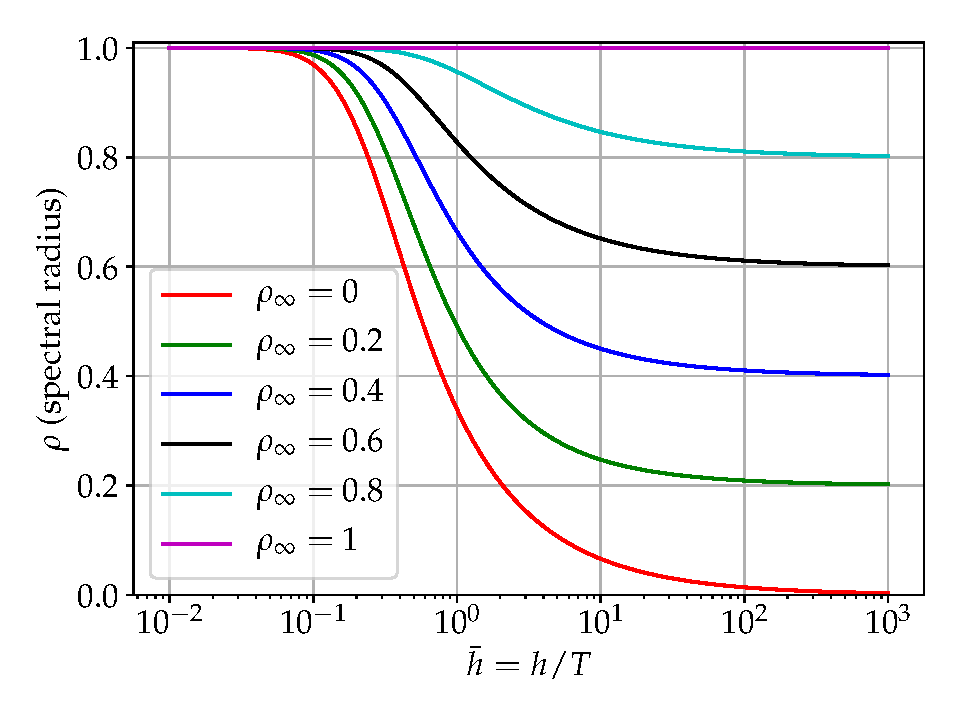
\includegraphics[width=0.6\columnwidth]{figures/spectralRadiusZeta0}%
\end{center}
\caption{Spectral radius for generalized-$\alpha$ method depending on dimensionless step size $\bar h=h/T$, in which
$T$ is the period of an equivalent single DOF mass-spring-damper system.}%
\label{fig:spectralRadius}%
\end{figure}


% ++++++++++++++++++++++++++++++++++++++++++++++++++++++++
% ++++++++++++++++++++++++++++++++++++++++++++++++++++++++
\mysubsubsection{Newton iteration}
\newcommand{\avu}{\ddot \qv} %unknown acceleration
%
\newcommand{\GA}{{G\alpha}} %abbreviation to mark equations, residuals, etc.
%
Thus, the residuals at the end of the time step ($T$) read (put all terms to LHS):
\bea \label{eq_generalizedAlphaRes}
  \rv^\GA_\SO &=& \Mm \ddot \qv_T + \frac{\partial \gv}{\partial \qv^\mathrm{T}} \tlambda_T - \fv_\SO(\qv_T, \dot \qv_T, t) = 0\\
  \rv^\GA_\FO &=& \dot \yv_T + \frac{\partial \gv}{\partial \yv^\mathrm{T}} \tlambda_T - \fv_\FO(\yv_T, t) = 0\\
	\rv^\GA_\AE &=& \gv(\qv_T, \dot \qv_T, \yv_T, \tlambda_T, t) = 0
\eea
%
We consider two options for \SON: (A) solve for unknown accelerations $\avu_T$,  or (B) for unknown displacements $\qv_T$.

\mysubsubsubsection{(A) Solve for unknown accelerations}
%
The unknowns for the Newton method then are
\be \label{eq_Newton_unknowns1}
  \txi^\GA_{k+1} = \vr{\avu_T}{\yv_T}{\tlambda_T}
\ee
and at the beginning of the step, we have
\be \label{eq_Newton_unknowns2}
  \txi^\GA_{k} = \vr{\avu_0}{\yv_0}{\tlambda_0}
\ee
For the Newton method, we need to compute an update for the unknowns of \eq{eq_Newton_unknowns1}, using the previous residual $\rv_{k}$ and the inverse of the Jacobian $\Jm_{k}$ of Newton iteration $k$,
\be
  \txi^\GA_{k+1} = \txi^\GA_{k} - \Jm^{-1} \left( \txi^\GA_{k} \right) \cdot \rv^\GA \left( \txi^\GA_{k} \right)
\ee

% +++++++++++++++++++++
% Jacobians for Newmark
The Jacobian has the following $3 \times 3$ structure,
\be
  \Jm = \mr{\Jm_{\SO\SO}}{\Jm_{\SO\FO}}{\Jm_{\SO\AE}}
           {\Jm_{\FO\SO}}{\Jm_{\FO\FO}}{\Jm_{\FO\AE}}
           {\Jm_{\AE\SO}}{\Jm_{\AE\FO}}{\Jm_{\AE\AE}}
			= \mr{\Jm_{\SO\SO}}{\Null}{\Jm_{\SO\AE}}
           {\Null}{\Jm_{\FO\FO}}{\Jm_{\FO\AE}}
           {\Jm_{\AE\SO}}{\Jm_{\AE\FO}}{\Jm_{\AE\AE}}
\ee
in which we consider $\Jm_{\FO\SO}$ and $\Jm_{\SO\FO}$ to vanish in the current implementations, which means that coupling of ODE1 and ODE2 coordinates is only possible due to algebraic equations.

The remaining terms in the Jacobian read
\bea
  \Jm_{\SO\SO}&=&\frac{\partial \rv^\GA_\SO}{\partial \avu} 
							 = \frac{\partial \rv^\GA_\SO}{\partial \qv} \frac{\partial \qv}{\partial \avu} 
							   + \frac{\partial \rv^\GA_\SO}{\partial \dot \qv} \frac{\partial \dot \qv}{\partial \avu} 
							 = h^2 \beta \Km + h \gamma \Dm
							 \nonumber \\
	\Jm_{\SO\AE}&=&\frac{\partial \rv^\GA_\SO}{\partial \tlambda} 
	             = \frac{\partial \gv}{\partial \qv} \quad (\mbox{or } \frac{\partial \gv}{\partial \dot \qv} \mbox{ for constraints at velocity level)} \nonumber \\
	\Jm_{\FO\FO}&=&\frac{\partial \rv^\GA_\FO}{\partial \yv} \nonumber \\
	\Jm_{\AE\SO}&=&\frac{\partial \rv^\GA_\AE}{\partial \avu}
	             = \frac{\partial \gv}{\partial \avu}
	             = \frac{\partial \gv}{\partial \qv} \frac{\partial \qv}{\partial \avu} + 
							   \frac{\partial \gv}{\partial \dot \qv} \frac{\partial \dot \qv}{\partial \avu}
							 = h^2 \beta \frac{\partial \gv}{\partial \qv} 
							   + h \gamma \frac{\partial \gv}{\partial \dot \qv}
							\nonumber \\
	\Jm_{\AE\FO}&=&\frac{\partial \rv^\GA_\AE}{\partial \yv} \nonumber \\
	\Jm_{\AE\AE}&=&\frac{\partial \rv^\GA_\AE}{\partial \tlambda}
							 = \frac{\partial \gv}{\partial \tlambda}
\eea
%
Once an update $\qv^\mathrm{Newton}_{k+1}$ has been computed, the interpolation formulas \eqref{eq_Newmark_interpolation} need to be evaluated before the next residual and Jacobian can be computed.
%
\mysubsubsubsection{(B) Solve for unknown displacements}
%
This approach is similar to the previous approach and follows exactly the algorithm given by Arnold and Br\"uls \cite{Arnold2007}, however, extended for ODE1 variables, which are integrated by the (undamped) trapezoidal rule.
Documentation will be added lateron.

\mysubsubsection{Initial accelerations}
%
For the solvers based on the implicit trapezoidal rule, initial accelerations are necessary in order to significantly increase the accuracy
of the first time step.
For this reason, the constraints $\gv(\qv_0, \dot \qv_0, \yv_0, \tlambda_0, t) = 0$ in \eq{eq_system_EOM} are differentiated w.r.t.\ time,
\be \label{eq_initialAccelerationsVel}
	\dot \gv(\qv_0, \dot \qv_0, \yv_0, \tlambda_0, t) = 
	\frac{\partial \gv}{\partial \qv} \dot \qv_0 + 
	\frac{\partial \gv}{\partial \dot \qv}\ddot \qv_0 +
	\frac{\partial \gv}{\partial \yv} \dot \yv_0 + 
	\frac{\partial \gv}{\partial \tlambda} \dot \tlambda +
	\frac{\partial \gv}{\partial t} = 0 \eqDot 
\ee
Currently, we assume $\frac{\partial \gv}{\partial \tlambda} = 0$ for all further derivations on initial accelerations.
For velocity level constraints, \eq{eq_initialAccelerationsVel} is used to extract initial accelerations $\ddot \qv_0$,
\be
  \frac{\partial \gv}{\partial \dot \qv}\ddot \qv_0 = %\Gm_{ia-vel} \ddot \qv_0 = \gv_{ia-vel}(\qv_0, \dot \qv_0, \yv_0, t) = 
	  -\frac{\partial \gv}{\partial \qv} \dot \qv_0 
		-\frac{\partial \gv}{\partial \yv} \dot \yv_0
	  %-\frac{\partial \gv}{\partial \tlambda} \dot \tlambda 
		-	\frac{\partial \gv}{\partial t} \eqDot
\ee
%
Finally, the equations for the computation of the initial accelerations read for velocity level constraints,
note that $\yv_{init}$ are the nodal initial values for $\yv$,
\be \label{eq_initialAccelerationsVel2}
  \mr{\Mm}{\Null}{\frac{\partial \gv}{\partial \dot \qv^\mathrm{T}}} 
	   {\Null}{\Im}{\Null}
		 {\frac{\partial \gv}{\partial \dot \qv}}{\Null}{\Null}
		 \vr{\ddot \qv_0}{\yv_0}{\tlambda_0}
   = \vr{\fv_\SO(\qv_T, \dot \qv_T, t)}{\yv_{init}}
	      {-\frac{\partial \gv}{\partial \qv} \dot \qv_0-\frac{\partial \gv}{\partial \yv} \dot \yv_0 - \frac{\partial \gv}{\partial t}}  \eqComma
\ee
%
The term $\frac{\partial \gv}{\partial t}$ can only occur in case of user functions and therefore currently not implemented, and the ODE1 term $\frac{\partial \gv}{\partial \yv} = 0$ is not used yet in constraints.

For position level constraints, we assume $\frac{\partial \gv}{\partial \dot \qv} = 0$ and $\frac{\partial \gv}{\partial \yv} = 0$ in \eq{eq_initialAccelerationsVel} and perform a second derivation w.r.t.\ time,
\be \label{eq_initialAccelerationsPos}
	\ddot \gv(\qv_0, \dot \qv_0, \yv_0, \tlambda_0, t) = 
	\frac{\partial^2 \gv}{\partial \qv^2} \dot \qv_0^2 + 
	2 \frac{\partial^2 \gv}{\partial \qv \partial t} \dot \qv_0 + 
	\frac{\partial \gv}{\partial \qv} \ddot \qv_0 + 
	%\frac{\partial^2 \gv}{\partial \yv^2} \dot \yv_0^2 + 
	%\frac{\partial \gv}{\partial \yv} \ddot \yv_0 + 
	\frac{\partial^2 \gv}{\partial t^2} = 0 \eqDot
\ee
For position level constraints, \eq{eq_initialAccelerationsPos} is used to extract initial accelerations $\ddot \qv_0$,
\be
  \frac{\partial \gv}{\partial \qv} \ddot \qv_0 = %\Gm_{ia-pos} \ddot \qv_0 = \gv_{ia-pos}(\qv_0, \dot \qv_0, \yv_0, t) = 
	- 2 \frac{\partial^2 \gv}{\partial \qv \partial t} \dot \qv_0
	- \frac{\partial^2 \gv}{\partial \qv^2} \dot \qv_0^2
	%- \frac{\partial^2 \gv}{\partial \yv^2} \dot \yv_0^2
	%- \frac{\partial \gv}{\partial \yv} \ddot \yv_0
	- \frac{\partial^2 \gv}{\partial t^2} \eqDot
\ee
Finally, the equations for the computation of the initial accelerations for position level constraints read
\be \label{eq_initialAccelerationsPos2}
  \mr{\Mm}{\Null}{\frac{\partial \gv}{\partial \qv^\mathrm{T}}} 
	   {\Null}{\Im}{\Null}
		 {\frac{\partial \gv}{\partial \qv} }{\Null}{\Null}
		 \vr{\ddot \qv_0}{\yv_0}{\tlambda_0}
   = \vr{\fv_\SO(\qv_T, \dot \qv_T, t)}{\yv_{init}}
	      {- 2 \frac{\partial^2 \gv}{\partial \qv \partial t} \dot \qv_0 - \frac{\partial^2 \gv}{\partial \qv^2} \dot \qv_0^2	- \frac{\partial^2 \gv}{\partial t^2}}  \eqComma
\ee
%in which $\gv_{ia}$ and $\Gm_{ia}$ are placeholder for either $\gv_{ia-pos}$ and $\Gm_{ia-pos}$ for position level constraints and $\gv_{ia-vel}$ resp.\ $\Gm_{ia-vel}$ for velocity level constraints.
The linear system of equations \ref{eq_initialAccelerationsVel2} or \ref{eq_initialAccelerationsPos2} is solved prior to an implicit time integration if 
\bi
  \item[] \texttt{simulationSettings.timeIntegration.generalizedAlpha.computeInitialAccelerations = True} 
\ei
which is the default value.
%
%The unknowns for the Newton method are
%\be \label{eq_Newton_unknowns}
  %\qv^\mathrm{Newton} = \vr{\avu^T_\SO}{\vel^T_\FO}{\qv^T_\AE}
%\ee
%For the Newton method, we need to compute an update for the unknowns \eq{eq_Newton_unknowns}, using the known residual $\rv_{i-1}$ and the inverse of the Jacobian $\Jm_{i-1}$ of step $i-1$,
%\be
  %\qv^\mathrm{Newton}_{i} = \qv^\mathrm{Newton}_{i-1} - \Jm^{-1}\left( \qv^\mathrm{Newton}_{i-1}\right) \rv\left( \qv^\mathrm{Newton}_{i-1}\right)
%%  \qv^\mathrm{Newton}_{i} = \qv^\mathrm{Newton}_{i-1} - \Jm^{-1}_{i-1} \Rm\left(\avu^T_{\SO,i-1},\,\vel^T_{\FO,i-1},\,\qv^T_{\AE,i-1} \right)
%\ee
%
%% +++++++++++++++++++++
%% Jacobians for Newmark
%The Jacobian has the following $3 \times 3$ structure,
%\be
  %\Jm = \mr{\Jm_{\SO\SO}}{\Jm_{\SO\FO}}{\Jm_{\SO\AE}}
           %{\Jm_{\FO\SO}}{\Jm_{\FO\FO}}{\Jm_{\FO\AE}}
           %{\Jm_{\AE\SO}}  {\Jm_{\AE\FO}}  {\Jm_{\AE\AE}}
%\ee
%Note that currently, all terms related to '$\FO$' are not implemented. The other terms are only evaluated in the specific jacobian computation, if according flags are set in GetAvailableJacobian(). 
%Otherwise, the constraint needs to be implemented as object which can employ all kinds of coordinates, which do not depend on coordinates of markers.
%
%The available Jacobians need to be rewritten in terms of the Newton unkowns \eqref{eq_Newton_unknowns}, and thus read
%\bea
  %\Jm_{\SO\SO}&=&\frac{\partial \fv^\mathrm{Newmark}_\SO}{\partial \avu_\SO^\mathrm{T}} 
							 %= \frac{\partial \fv^\mathrm{Newmark}_\SO}{\partial \qv_\SO^\mathrm{T}} \frac{\qv_\SO}{\avu_\SO^\mathrm{T}} 
							   %+ \frac{\partial \fv^\mathrm{Newmark}_\SO}{\partial \dot \qv_\SO^\mathrm{T}} \frac{\dot \qv_\SO}{\avu_\SO^\mathrm{T}} 
							 %= h^2 \beta \Km + h \gamma \Dm
							 %\nonumber \\
	%\Jm_{\SO\AE}&=&\frac{\partial \fv^\mathrm{Newmark}_\SO}{\partial \qv_\AE^\mathrm{T}} 
	             %= \frac{\partial \gv}{\partial \qv_\SO^\mathrm{T}} \nonumber \\
	%\Jm_{\AE\SO}&=&\frac{\partial \fv^\mathrm{Newmark}_\AE}{\partial \avu_\SO^\mathrm{T}} 
	             %= \frac{\partial \gv}{\partial \avu_\SO^\mathrm{T}}
	             %= \frac{\partial \gv}{\partial \qv_\SO^\mathrm{T}} \frac{\qv_\SO}{\avu_\SO^\mathrm{T}} + \frac{\partial \gv}{\partial \dot \qv_\SO^\mathrm{T}} \frac{\dot \qv_\SO}{\avu_\SO^\mathrm{T}}
							 %= h^2 \beta \frac{\partial \gv}{\partial \qv_\SO^\mathrm{T}} 
							   %+ h \gamma \frac{\partial \gv}{\partial \dot \qv_\SO^\mathrm{T}}
							%\nonumber \\
	%\Jm_{\AE\AE}&=&\frac{\partial \fv^\mathrm{Newmark}_\AE}{\partial \qv_\AE^\mathrm{T}}
							 %= \frac{\partial \gv}{\partial \qv_\AE^\mathrm{T}}
%\eea
%Note that the derivative $\frac{\qv_\SO}{\avu_\SO^\mathrm{T}}$ follows from the Newmark interpolation \eqref{eq_Newmark_interpolation} using the relation between $\qv^T_\SO$ and $\avu^T_\SO$. The tangent stiffness matrix $\Km$ must also include derivatives of applied forces $\fv^a$, which is currently not implemented.
%Furthermore, the Jacobian is not symmetric, which could be obtained by according scaling.

%
% +++++++++++++++++++++
% Newton update formula
%Once an update $\qv^\mathrm{Newton}_{k+1}$ has been computed, the interpolation formulas \eqref{eq_Newmark_interpolation} need to be evaluated before the next residual and Jacobian can be computed.

%\mysubsubsection{Jacobian computation}
%
%The computation of the global jacobian matrix is time consuming for the static solver or implicit time integration.
%The equations are split into \SON, \FON and \AEN parts. From this structure, in the general non-symmetric case, 3 $\times$ 3 submatrices result for the jacobian.
%Every submatrix of the jacobian has a certain meaning and needs to be computed individually.
%Specifically, in implicit time integration the \SON $\times$ \SON term includes the (tangent) stiffness matrix and the mass matrix.
%
%For efficient computation purpose, the elements provide a list of flags, which determine the dependencies as well as available (analytical) functions to compute the local (object) jacobian:
%\bi
  %\item ODE2\_ODE2 $\ldots$ derivative of ODE2 equations with respect to ODE2 variables
  %\item ODE2\_ODE2\_t $\ldots$ derivative of ODE2 equations with respect to ODE2\_t (velocity) variables
  %\item ODE1\_ODE1 $\ldots$ derivative of ODE1 equations with respect to ODE1 variables (NOT YET AVAILABLE)
  %\item AE\_ODE2 $\ldots$ derivative of AE (algebraic) equations with respect to ODE2 variables
  %\item AE\_ODE2\_t $\ldots$ derivative of AE (algebraic) equations with respect to ODE2\_t (velocity) variables (NOT YET AVAILABLE)
  %\item AE\_ODE1 $\ldots$ derivative of AE (algebraic) equations with respect to ODE1 variables (NOT YET AVAILABLE)
  %\item AE\_AE $\ldots$ derivative of AE (algebraic) equations with respect to AE variables
%\ei
%If one of these flags is set (binary; e.g.ODE2\_ODE2 + ODE2\_ODE2\_t), then the according local jacobian is computed and assembled into the global jacobian in the static or implicit dynamic solver.
%
%Jacobians can also be supplied in analytical (function) form, which is indicated by an additional flag with the same name but an additional term '\_function', e.g.\ 'ODE2\_ODE2\_function' indicates that the derivative of ODE2 equations with respect to its ODE2 coordinates is provided in an analytical form (this is the tangent stiffness matrix).
%
%Two {\bf object} functions are used to compute the local jacobians:
%\bi
  %\item \texttt{\bf ComputeJacobianODE2\_ODE2(Matrix\& jacobian, Matrix\& jacobian\_ODE2\_t)}: computes the \texttt{ODE2\_ODE2} and \texttt{ODE2\_ODE2\_t} jacobians
	%\item \texttt{\bf ComputeJacobianAE(Matrix\& jacobian, Matrix\& jacobian\_AE)}: computes the \texttt{AE\_ODE2} and \texttt{AE\_AE} jacobians of the object ITSELF
%\ei
%Two {\bf connector} functions are used to compute the local jacobians, using \texttt{MarkerData}:
%\bi
  %\item \texttt{\bf ComputeJacobianODE2\_ODE2(Matrix\& jacobian, Matrix\& jacobian\_ODE2\_t, const MarkerDataStructure\& markerData)}: computes the \texttt{ODE2\_ODE2} and \texttt{ODE2\_ODE2\_t} jacobians of the connector; e.g.\ for spring-damper
	%\item \texttt{\bf ComputeJacobianAE(Matrix\& jacobian, Matrix\& jacobian\_AE, const MarkerDataStructure\& markerData)}: computes the \texttt{AE\_ODE2} and \texttt{AE\_AE} jacobians of the connector; e.g.\ for coordinate constraint
%\ei
%
%The system jacobian has the structure (\SO = ODE2, \FO = ODE1, $\AE$ = AE; $\bar \fv_\SO$ = according system residual including dynamic (mass matrix) terms in time integration; $\gv_\AE$ = algebraic equations):
%\be
  %\bigmr
  %{\frac{\partial \bar \fv_\SO}{\partial \qv_\SO}} {0} {\left(\frac{\partial \gv_\AE}{\partial \qv_\SO}\right)^T}
  %{0} {\frac{\partial \fv_\FO}{\partial \qv_\FO}} {\left(\frac{\partial \gv_\AE}{\partial \qv_\FO}\right)^T}
	%{\frac{\partial \gv_\AE}{\partial \qv_\SO}} {\frac{\partial \gv_\AE}{\partial \qv_\FO}} {\frac{\partial \gv_\AE}{\partial \qv_\AE}}
%\ee
%
%Two system jacobian functions are currently available:
%\bi
  %\item \texttt{\bf JacobianODE2RHS(temp, newton, factorODE2, factorODE2\_t, jacobian\_ODE2, jacobian\_ODE2\_t)}: compute analytical/numerical differentiation of ODE2RHS w.r.t. ODE2 and ODE2\_t coordinates; if analytical/functional version of jacobian is available and Newton flag 'useNumericalDifferentiation'=false, then the according jacobian is computed by its according function; results are 2 jacobians; the factors 'factor\_ODE2' and 'factor\_ODE2\_t' are used to scale the two jacobians; if a factor is zero, the according jacobian is not computed.
	%\item \texttt{\bf JacobianAE(temp, newton, jacobian, factorODE2, velocityLevel, fillIntoSystemMatrix)}: 
		%compute constraint jacobian of AE with respect to ODE2 ('fillIntoSystemMatrix'=true: also w.r.t. [ODE1] and AE) coordinates $\ra$ direct computation given by access functions; 'factorODE2' is used to scale the ODE2-part of the jacobian (to avoid postmultiplication); velocityLevel = true: velocityLevel constraints are used, if available; 'fillIntoSystemMatrix'=true: fill in both $\frac{\partial \bar \fv_\AE}{\partial \qv_\SO}$, $\frac{\partial \bar \fv_\AE}{\partial \qv_\SO}^T$ AND $\frac{\partial \bar \fv_\AE}{\partial \qv_\AE}$ at according locations into system matrix; 'fillIntoSystemMatrix'=false: (this is a temporary/WORKAROUND function):
%\ei
%The system jacobian functions compute the local jacobians either by means of a provided function or numerically, using the 'NumericalDifferentiation' settings of 'Newton'.
%




%++++++++++++++++++++++++++++++++++++++++++++++++++++++++++++++++++++++++++
%++++++++++++++++++++++++++++++++++++++++++++++++++++++++++++++++++++++++++
%++++++++++++++++++++++++++++++++++++++++++++++++++++++++++++++++++++++++++
\newpage
\mysubsection{Optimization and parameter variation}
%
The real benefit of powerful multi-body simulation emerges only if combined with modern but also simple analysis and evaluation methods.
Therefore, \codeName\ has been integrated into the Python language, which offers a virtually unlimited number of methods of post-processing, evaluation and optimization.
In this section, two methods that are directly integrated into \codeName\ are revisited.
%
\label{sec:parameterVariation}
\mysubsubsection{Parameter Variation}
Parameter variation is one of the simplest tools to evaluate the dependency of the solution of a problem on certain parameters. This usually requires the computation of an objective (goal, result) value for a single computation (e.g, some error norm, maximum vibration amplitude, maximum stress, maximum deflection, etc.) for every computation. Furthermore, it needs to be run for a set of parameters, e.g., using a \texttt{for} loop.
While this could be done manually in \codeName , it is recommended to use built-in functions, which simplify evaluation and postprocessing and directly enable parallelization.
The according function \texttt{ParameterVariation(...)}, see \refSection{sec:processing:ParameterVariation}, performs a set of multi-dimensional parameter variations using a dictionary that describes the variation of parameters. See also \texttt{parameterVariationExample.py} in the \texttt{Examples} folder for a simple example showing a 2D parameter variation. The function \texttt{ParameterVariation(...)} requires the \texttt{multiprocessing} Python module which enables simple multi-threaded parallelism and has been tested for up to 80 cores on the LEO4 supercomputer at the University of Innsbruck, achieving a speedup of 50 as compared to a serial computation.

\mysubsubsection{Genetic Optimization}
\label{sec:optimization}
%
In engineering, we often need to find a set of unknown, independent parameters $\xv \in \Rcal^n$, $\xv$ being denoted as design variables and $\Rcal^n$ as design space. Sometimes, the design space is further subjected to constraints $\gv(\xv)=0$ as well as inequalities $\hv(x) \le 0$, which are not considered here. For simple solutions for constrained optimization problems using penalty methods, see the introductory literature \cite{Kiusalaas2013}.

Optimization problems are written in general in the form
\be
  \min\limits_{\xv} f(\xv), \quad \xv \in \Rcal^n \eqComma
\ee
where $f(\xv)$ denotes the {\it objective function} (={\it fitness function}). If we would like to maximize a function $\bar f(\xv)$, simply set $f(\xv)=-\bar f(\xv)$.

In engineering, the optimization problem could seek model parameters, e.g., the geometric dimensions and inertia parameters of a slider crank mechanism, in order to achieve smallest possible forces at the supports.
Another example is the identification of unknown physical parameters, such as stiffness, damping of friction. This can be achieved by comparing measurement and simulation data (e.g., accelerations measured at relevant parts of a machine). Lets assume that $\epsilon(t)$ is an error computed in every time step of a computation, then we can set the objective (=fitness) function, e.g., as 
\be
  f(x) = \frac 1 T \sqrt{\int_{t=0}^T \epsilon(t)^2 dt}
\ee
as the integral over the error $\epsilon$ between measurement and simulation data.
In general, a parameter variation would be sufficient to compute sufficient computations for all combinations within the design space, however, a 3D design space with 100 variations into every direction (e.g., varying the unknown damping coefficient between 1 and 100, etc.) would already require 1000.000 computations, which in an ideal case of 1 second/computation leads to almost 2 weeks of computation time.

As an alternative stochastic methods can be use to compute only the objective function for a smaller set of randomly generated design variables, which usually show regions with better parameters (lower $f$) in scatter plots.

{\bf Genetic algorithms}\cite{Goldberg1989, Whitley1994} can significantly reduce the necessary amount of objective function evaluations in order to perform the optimization. Genetic identification algorithms have been already successfully applied to multibody system dynamics\cite{Eder2014}. 

The general structure of a (canonical) genetic algorithm is depicted in \fig{fig_geneticOptimization}.
%++++++++++++++++++++++++++++++++++++++++++++++++++++++++++++++++++++++++
\begin{figure}[hb]
  \centering
	\begin{tikzpicture}[node distance = 2cm, auto, thick,scale=0.7, every node/.style={scale=0.7}]
			% Place nodes
			\node [cloud] (geneticOptimization) {\texttt{GeneticOptimization(...)}};
%			\node [wideblock, below of=init_solver_specific] (initializeSolver) {InitializeSolver()};
			\node [wideblock, below of=geneticOptimization, node distance=2cm] (initial) {1.\ create initial population $S_i$ with $n_{pi}$ individuals};
			\node [wideblock, below of=initial, node distance=2.5cm] (fitness) {2.\ evaluate fitness for population};
			\node [wideblock, below of=fitness] (surviving) {3.\ select (surviving) individuals $S_s$};
			\node [wideblock, below of=surviving] (crossover) {4.\ create crossover population $S_c$};
			\node [wideblock, below of=crossover] (mutation) {5.\ create mutated population $S_m$};
			\node [decision, below of=mutation, node distance=3cm] (decision) {6.\ fitness goal or number of generations $n_g$ not reached?};
			\node [wideblock, below of=decision, node distance=3.5cm] (end) {END};
			%
			\path [arrow] (geneticOptimization) -- (initial);
			\path [arrow] (initial) -- (fitness);
			\path [arrow] (fitness) -- (surviving);
			\path [arrow] (surviving) -- (crossover);
			\path [arrow] (crossover) -- (mutation);
			\path [arrow] (mutation) -- (decision);
			\path [arrow] (decision) -- node [near start] {False} +(6cm,0) |- (fitness);
			%(D.west) -- +(-1,0) |- node[pos=0.25] {No} (C);
			\path [arrow] (decision) -- node [near start] {True}(end);
	\end{tikzpicture}
  \caption{Basic solver flow chart genetic algorithm / optimization.}
	\label{fig_geneticOptimization}
\end{figure}
%
%\bn\setlength{\itemindent}{0.5cm}
  %\item START
  %\item create initial population $n_{pi}$
	%\item evaluate fitness for population\footnote{This is usually the time consuming part, which requires a single simulation run for every fitness evaluation}
	%\item select (surviving) individuals $S_s$
	%\item crossover $S_c$
	%\item mutation $S_m$
	%\item if fitness goal or number of generations $n_g$ not reached, continue with step
	%\item END
%\en
For details, see the cited literature. Here, we focus on the implementation of the function 
\texttt{GeneticOptimization(...)}, see \refSection{sec:processing:GeneticOptimization}.
The initial population (step 1) is created with \texttt{initialPopulationSize} individuals with uniformly distributed random design variables $[\xv_0, \ldots, \xv_{n_{pi}-1}]$\footnote{$\xv_i=[x_{i0}, x_{i1}, \ldots]$ being a set of genes, with single genes $x_{i0}$, $x_{i1}$, ... } in the search space, which is given in the dictionary \texttt{parameters}. Herafter (steps 2-6), we iteratively process a population for a certain \text{numberOfGenerations} generations.

In step 3, the surviving individuals $S_s$ with best fitness (smallest value from evaluation of \texttt{objectiveFunction}) are selected and considered further in the optimization. If the \texttt{distanceFactor} is used, the surviving individuals must be located within a certain distance (measured relative to the range of the search space) to all other surviving individuals. This option guarantees the search within several local minima, while a conventional search often converges to one single minimum.
Crossover (step 4)  is performed using a crossover of all available parameters of two randomly selected parents when generating children from the surviving individuals. The crossover of genes is performed only for a part of the new population, defined by \texttt{crossoverAmount}.

Finally, in step 5, we apply mutation to all genes, which extends the search to the surrounding design space of the individuals created by crossover. The mutation could be performed by means of certain distribution functions in order to focus on the currently best search regions. However, in the current implementation of \texttt{GeneticOptimization(...)} we simply use a uniform random variable to distribute the genes over a certain percentage of the design space, which is reduced in every generation defined by the \texttt{rangeReductionFactor} $r_r$. This allows us to restrict further search to a smaller subregion of the design space and in general allows a reduction of search space by means of $r_r^{n_g}$. In the ideal case, using sufficiently large population sizes and being lucky with the found random values, a range reduction factor $r_r=0.7$ reduces the search space by a factor of $100$ after every 13 generations, allowing to obtain 4 digits of accuracy for design variables after 26 generations for suitable optimization problems.

It should be noted that still this optimization method is based on random values and thus may fail occasionally for any problem case. In order to get reproducible results, set \texttt{randomizerInitialization} to any integer value (simply: 0) in order to get identical results for repeated runs. Setting the latter variable guarantees that the Python (numpy) randomizer creates the same series of random values for initial population, mutation, etc.




